\documentclass[tikz, border = 5pt]{standalone}

\usepackage{amsmath}
\usepackage{amsfonts}
\usepackage{amssymb}
\usepackage{graphicx}
\usepackage{tikz}
\usetikzlibrary{decorations.pathreplacing}
\usetikzlibrary{decorations.text}
\usetikzlibrary{positioning, fit, arrows,shapes,backgrounds, shadows,fadings,trees}

%\usetikzlibrary{intersections}
\usetikzlibrary{calc}
\usepackage{lmodern}

\usepackage[T1]{fontenc}

\definecolor{cA}{RGB}{143,136,190}
\definecolor{cB}{RGB}{51,103,172}

\begin{document}



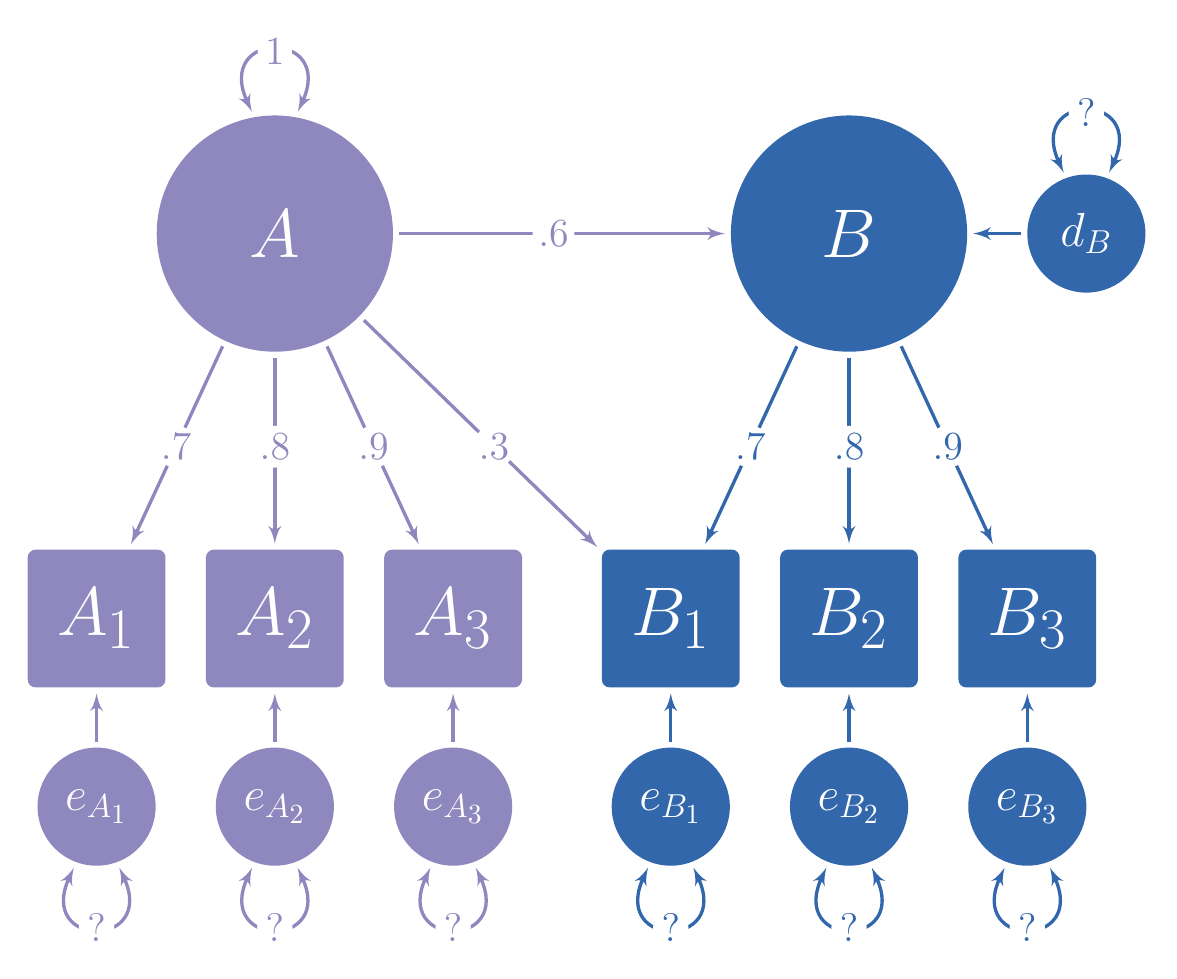
\begin{tikzpicture}[scale=1,  
latent/.style={circle, fill = gray, minimum size = 3cm, align = center,inner sep = 0cm,font = \fontsize{45}{60}\selectfont, text = white},
error/.style={circle, fill = gray, inner sep=1mm, minimum size=1.5cm, font=\LARGE, text = white},
ob/.style={rectangle, fill = gray,inner sep=2mm, minimum width=1.75cm, minimum height=1.75cm, align=center, rounded corners=0.1cm,font=\Huge, text = white},
post/.style={->,draw,shorten >=2pt,shorten <=2pt,>=latex', very thick, font=\LARGE, color = gray!70},
cov/.style={<->,draw,shorten >=2pt,shorten <=2pt,>=latex', color = gray!70, looseness=1.3, very thick, font=\large, bend left=50},
variance/.style={<->,  >=latex', draw, very thick, bend left=245, looseness=6,shorten >=2pt,shorten <=2pt, font=\Large, color = gray!70},
upvariance/.style={<->,  >=latex', thick, shorten >=2pt,shorten <=2pt, font=\Large,bend left = 115,looseness=4},
label/.style={fill=white,circle,inner sep = 0.1mm,font = \Large},
A/.style = {cA},
B/.style = {cB}]

\node[ob, fill = cA] (A1) {$A_1$};
\node[ob, right = 0.5cm of A1, fill = cA] (A2) {$A_2$};
\node[ob, right = 0.5cm of A2, fill = cA] (A3) {$A_3$};
\node[ob, right = 1cm of A3, fill = cB] (B1) {$B_1$};
\node[ob, right = 0.5cm of B1, fill = cB] (B2) {$B_2$};
\node[ob, right = 0.5cm of B2, fill = cB] (B3) {$B_3$};



\node[latent, above = 2.5cm of A2, fill = cA] (A) {$A$}; 
\node[latent, above = 2.5cm of B2, fill = cB] (B) {$B$}; 

\path[post, cA] (A)  to node[label, pos = 0.475]{.6} (B);


\path (A) to coordinate[pos = .48](center)   (A2);

\coordinate (l1) at (center -| A1); 
\coordinate (l2) at (center -| B3);

\path[post, cA] (A)  to (A1);
\path[post, cA] (A)  to (A2);
\path[post, cA] (A)  to (A3);
\path[post, cA] (A) to  (B1);

\path[post, cB] (B)  to (B1);
\path[post, cB] (B)  to (B2);
\path[post, cB] (B)  to (B3);
\node[label, text = cA] at (intersection of l1--l2 and A--A1) {.7};
\node[label, text = cA] at (intersection of l1--l2 and A--A2) {.8};
\node[label, text = cA] at (intersection of l1--l2 and A--A3) {.9};
\node[label, text = cA] at (intersection of l1--l2 and A--B1) {.3};
\node[label, text = cB] at (intersection of l1--l2 and B--B1) {.7};
\node[label, text = cB] at (intersection of l1--l2 and B--B2) {.8};
\node[label, text = cB] at (intersection of l1--l2 and B--B3) {.9};



\foreach \i in {1,2,3} {
	\node[error, below = 0.75cm of A\i, fill = cA] (eA\i) {$e_{A_\i}$};
	\node[error, below = 0.75cm of B\i, fill = cB] (eB\i) {$e_{B_\i}$};
	\path[variance, cA] (eA\i.250) to node[label]{?} (eA\i.290);
	\path[variance, cB] (eB\i.250) to node[label]{?} (eB\i.290);
	\path[post, cA] (eA\i) to (A\i);
	\path[post, cB] (eB\i) to (B\i);
}

\path[variance, cA] (A.80) to node[label]{1} (A.100);



\node[error, right = 0.75cm of B, fill = cB] (dB) {$d_{B}$};

\path[post, cB] (dB) to (B);
\path[variance, cB] (dB.70) to node[label]{?} (dB.110);

%\node (s) [below = of Gt]{};
%\node (n) [above = of Motor]{};
%\node (w) [left = of Power]{};
%\node (e) [right = of hex.east]{};
\end{tikzpicture}







\end{document}

